\documentclass{article}

\usepackage[
  paperheight=11in,
  paperwidth=8.5in,
  margin=1in]{geometry}
\usepackage{fontspec}
\setmainfont[Scale=1.25]{Liberation Sans}
\setmonofont[Scale=1.1]{Liberation Mono}
\usepackage[utf8]{inputenc}

\usepackage{graphicx}
\usepackage{wrapfig}
\usepackage[bottom]{footmisc}
\usepackage{listings}
\usepackage{enumitem}

\usepackage{wrapfig}
\usepackage{ragged2e}

\usepackage{array}
\usepackage[table]{xcolor}
\usepackage{multirow}
\usepackage{booktabs}
\usepackage{hhline}
\definecolor{palegreen}{rgb}{0.6,0.98,0.6}

\usepackage{amsmath}
\usepackage{amssymb}
\usepackage{multicol}
\usepackage{lipsum}
\usepackage{hyphenat}
\PassOptionsToPackage{hyphens}{url}
\usepackage{url}

\usepackage{rotating}

%\usepackage{xeCJK}

%% support use of straight quotes in code listings
\usepackage{listings}
\lstset{upquote=true}

%% for shrinking space between lines
\usepackage{setspace}
\onehalfspacing

\newcommand*{\affaddr}[1]{#1} % No op here. Customize it for different styles.
\newcommand*{\affmark}[1][*]{\textsuperscript{#1}}
\newcommand*{\email}[1]{\small{\texttt{#1}}}
\newcommand{\tarot}{\textsc{Tarot}}
\renewcommand*\contentsname{\centering Table of Contents}

\renewcommand{\footnoterule}{%
  \kern -3pt
  \hrule width \textwidth height 0.5pt
  \kern 2pt
}

% remove date
\date{}

\usepackage{titlesec}
\titleformat*{\section}{\large\bfseries}
\titleformat*{\subsection}{\normalsize\bfseries}
\titleformat*{\subsubsection}{\normalsize\bfseries}

\usepackage{biblatex}

\usepackage{hyperref}

\addbibresource{refs.bib}

\title{Good Enough: Facing the Cost-Performance Tradeoff for LLMs in Computing Education\footnote{\protectCopyright \copyright 2026. This is the author's version of the work. It is posted here by permission of CCSC for your
personal use. Not for redistribution. The definitive version will be published in The Journal of Computing Sciences in
Colleges (in press), ( 42, 5, 2026 Southeastern ), https://dl.acm.org/”.
}
}

\author{
Nicholas Gardella\\
Department of Computer Science\\
Washington and Lee University\\
Lexington, VA 24450\\
\email{ngardella@wlu.edu}\\
}

\begin{document}
\maketitle

\begin{abstract}
Perspectives on LLMs in CS education (e.g. \cite{falknerEffectiveUseLarge2026}) often rest on an assumption that human educators are more reliable curators of correct educational information for students than LLMs. This motivates restriction of LLM use for fielding student questions or providing grading feedback, for example. It also motivates the creation of deterministic software that can increase the reliability of LLMs, such as documentation lookup tools\footnote{e.g. Context 7 (\url{https://context7.com/})} that source reliable context to use as a basis for LLM generation. However, framing LLMs as generally unreliable has the downside to encourage \emph{disuse}, the ``neglect or underutilization of automation'' \cite{parasuramanHumansAutomationUse1997}. Informational resources are typically not unlimited. Libraries hold finite copies of books, instructors have limited time, and computers incur costs to operate. As such, frugal use helps for all users (students in this case) to get their share. Framing LLMs as unreliable \emph{should} discourage use and preserve resources. Instead, it can do quite the opposite. This proposal paper explains the LLM cost-performance tradeoff for computing educators using a practical example and a list of concrete recommendations for pedagogy, concluding with calls for needed future work.
\end{abstract}

\section{Introduction}\label{introduction}

Large Language Models (LLMs) are well suited to computer programming and educational applications \cite{pratherHypeComprehensiveReview2025}, but they are imperfectly reliable, creating potential harms for students \cite{falknerEffectiveUseLarge2026,pratherRobotsAreHere2023,wangLargeLanguageModels2025,zhouTeachersAreConfused2024a}. Computing students are increasingly using LLMs for educational help-seeking \cite{houEffectsGenerativeAI2024}, so educators need protective yet realistic messaging on this topic. Though the perspectives of students and instructors differ \cite{zastudilGenerativeAIComputing2023}, both parties show deep concerns about the real possibility for the LLMs they use to hallucinate and provide untrustworthy information \cite{pratherRobotsAreHere2023}. This has motivated researchers to suggest educational integrations of LLMs that cope with their unreliability \cite{falknerEffectiveUseLarge2026}. However, excessive focus on the unreliability of LLMs contributes to wasteful spending of the limited resources that enable them. This proposal paper challenges the unreliability narrative through the lens of the cost-performance tradeoff \cite{dingHybridLlmCostefficient2024}, promoting the use of less reliable models to promote economic and environmental stewardship \cite{renReconcilingContrastingNarratives2024}. After a realistic educational help-seeking example to illustrate this tradeoff, the primary contribution is a roadmap for how and why to adopt worse LLMs in computing education.

\begin{figure}
\centering
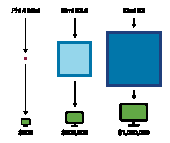
\includegraphics[width=3.5in]{figures/size-compare-phi-4-mini-kimi-k2.6-k3-on-priced-computers}
\caption{Scale diagram comparing a 4B LLM to larger 1.1T and 2.8T alternatives.}
\label{fig:scale-diagram}
\end{figure}

Note: Rectangle areas show, to scale, the relative data size of the numerical weights and biases that are the substance of an LLM. Reasonable estimates for the cost of the computing hardware required to run such models (in 2026 U.S. dollars) are provided. In reality, the Kimi models would not run on a single computer but rather many cooperating computers having the noted value in total.

\section{Background}\label{background}

\subsection{Cost-Performance Tradeoff}\label{cost-performance-tradeoff}

LLMs compress insights about their training data into a non-deterministic prediction machine embodied as a collection of numerical weights and biases. All else being equal, larger LLMs are more reliable than smaller ones but are also more expensive---computationally, financially, and environmentally \cite{dingHybridLlmCostefficient2024,renReconcilingContrastingNarratives2024}. This is because large LLMs need advanced computer hardware with high energy requirements to run effectively. \autoref{fig:scale-diagram} shows the relative data size (i.e., the volume of 0s and 1s that need to fit into the computer hardware) for three modern LLMs (in 2026). The larger ones, Moonshot AI's Kimi K2.6\footnote{\url{https://huggingface.co/moonshotai/Kimi-K2.6}} and K3\footnote{\url{https://huggingface.co/moonshotai/Kimi-K3}}, come in at 2.8 and 1.1 trillion parameters respectively, while the smaller, Microsoft's Phi 4 Mini\footnote{\url{https://huggingface.co/microsoft/Phi-4-mini-instruct}}, has just 4 billion parameters. All three models are open-weight, meaning anyone can freely download and run them on their own computer, but size can be practically prohibitive. Phi's parameters occupy a few gigabytes, requiring a modestly powerful consumer-grade computer to run, but the Kimi models require multiple terabytes, demanding high-performance clusters of industrial grade computers.

\subsection{Environmental and Social Motivations}\label{environmental-and-social-motivations}

Training and running LLMs is computationally intensive, so excessive reliability is wasteful. Computers incur substantial monetary cost and strain on the natural environment by using water and energy, much of which generates environmentally harmful carbon emissions \cite{dingHybridLlmCostefficient2024,renReconcilingContrastingNarratives2024,ModelRoutingAI}. Savings of money and natural resources cooperate nicely (e.g., saving energy saves money). Unfortunately, cost minimization can also encourage describing human workers in terms of their water, energy, and money usage compared to LLMs that can simulate their labor \cite{renReconcilingContrastingNarratives2024}. While out of scope here, critiquing this narrative within computing education is an important area for future work. What cost minimization gets right is that excess is wasteful. As the old idiom goes, \emph{you ought not} \emph{use a sledgehammer to crack a nut} \cite{judsonSagesHeroesAmerican1851}. Just the same, LLM users ought not use larger, more reliable LLMs if smaller, cheaper ones are just as reliable for the task at hand.

Smaller LLMs are also better for promoting equitable computing. Due to the costly computing needs of frontier LLMs (i.e. the largest, most reliable models of the day), control over these resources becomes centralized, even when model weights are open. LLM-based coding tools like GitHub Copilot, for example, offer users discounts to use an automatic model selector that prevents popular models from being overused \cite{CopilotAutoModel}. By controlling the means of intellectual production, large Artificial Intelligence (AI) providers exert a centralized social control over individual programmers \cite{sunyaevIdeologyDesignPurposeful2026}. This pattern contrasts the democratic spirit of computer programming, which traditionally allowed individuals to build path-breaking technology with minimal capital resources (i.e., money and equipment). Centralized corporate control also threatens computing education because it creates financial barriers for students to participate in computing at the cutting edge \cite{universityofnewsouthwalesExploringIntersectionDigital2020}. If computing educators embrace small, less reliable LLMs, this not only prevents waste but also preserves the democratic, enterprising spirit of computing for students who want and need to use LLMs but cannot afford frontier options.

\subsection{Existing Approaches}\label{existing-approaches}

AI providers are using intelligent model routing to prevent waste in LLM inference. Though training LLMs accounts for a huge portion of their cost \cite{moslemDynamicModelRouting2026,renReconcilingContrastingNarratives2024}, the present scope is focused on LLM inference, the stage where a given trained model is used repeatedly to service users' prompts. A core challenge with the cost-performance tradeoff is that LLMs are random by nature, so guessing how well they will perform is hard. However, AI researchers have developed intelligent strategies for routing and cascading users' prompts to prevent waste \cite{dingHybridLlmCostefficient2024,CopilotAutoModel,moslemDynamicModelRouting2026,ModelRoutingAI}. For example, a model can be trained to guess which of a set of increasingly reliable options will produce a response that is good enough for a given prompt \cite{dingHybridLlmCostefficient2024}. As long as that prediction model is efficient, it saves cost by only using a more powerful model when needed. Another technique, cascading, involves a guess-and-check strategy, where an efficient response evaluator \cite{zhangBERTScoreEvaluatingText2020} can test the output of a small LLM, escalating to larger ones until the response is good enough \cite{moslemDynamicModelRouting2026}. Overall, there is great promise in automatically choosing LLMs that best balance reliability with cost.

Automatic model selection only works if more powerful LLMs are available when needed, so computing educators are exploring ways to meet their needs with only small LLMs. LLMs can simulate complex generation tasks that traditionally involve planning, reasoning, and multiple subtasks. More powerful LLMs can often do such tasks without additional tools, obviating the need to provide any. For example, a large frontier LLM might be able to retrieve a given fact solely out of its parameters, while a smaller LLM might be able to do so only if given a web search tool to use for context. As a result, some computing education researchers advocate for giving LLMs specified sub-tasks (e.g. summarizing compiler error messages or lists of search results) rather than broad objectives \cite{falknerEffectiveUseLarge2026}. LLMs tend to perform better on narrower tasks, so small LLMs get huge reliability gains when used in this manner. For example, researchers have used multi-stage curation techniques with small LLMs to generate programming problems of similar quality to ones produced at baseline by large LLMs \cite{jimenezrodriguezPersonalizedCodingProblem2026}. Given students are using LLMs for help seeking \cite{houEffectsGenerativeAI2024}, other work has arranged small, specialized LLMs into personalized AI learning tools for students to approximate the performance of larger LLMs \cite{tanejaAgenticRAGPersonalized2025}. This promising area of work encourages resourceful stewardship of LLM technology while preserving the high reliability desired in education.

\section{Educational Example}\label{educational-example}

\begin{figure}
\centering
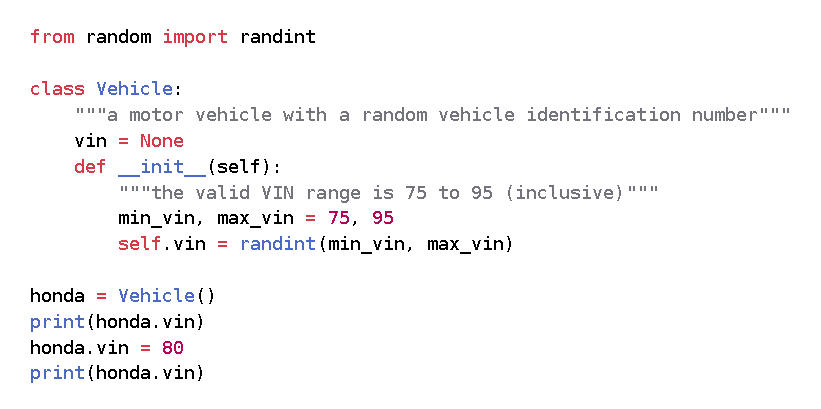
\includegraphics[width=\linewidth]{figures/python-vehicle-class-fictional-student-code}
\caption{Code attachment to a fictional student question.}
\label{fig:code-snippet}
\end{figure}


Next, the cost-performance tradeoff is examined through a case study of how two 2026 LLMs answer a fictional student question. In this scenario, Devin, a second-year university student, has come to office hours at the end of the first week of a second course in introductory computer science (CS2). Devin's CS1 course was taught in Python, but CS2 is taught in Java. Her question goes something like this (see \autoref{fig:scale-diagram} for her attached code):

\begin{quote}
In my Python course, I made a vehicle class where the VIN field was editable from outside the class code; can I do that in Java?
\end{quote}

There are many ways for Devin to obtain an answer: (1) ask the instructor, (2) research the question at a public library\footnote{Note: internet search was excluded, as search engines are increasingly using LLM-based features}, (3a) input the question to a powerful, frontier LLM (e.g., Kimi 2.6; see \autoref{fig:scale-diagram}), and (3b) input the question to a basic, accessible LLM (e.g., Phi 4 Mini; see \autoref{fig:scale-diagram}). As explained in \autoref{cost-performance-tradeoff}, Kimi is more reliable than Phi, but Phi is cheaper.

Option (1), asking the instructor, could be nerve-wracking for the student, but would provide an effective and inviting social opportunity to resolve the concern \cite{fanImpactAIassistedPair2025,gardellaHBCUStudentPerspectives2025}. The library, option (2), ought to have the most reliable information on the topic, provided it carries two relevant texts on Python and Java programming. A social interaction there would feature the same tension of vulnerability and pleasantness as with the instructor, but the librarian is unlikely to be an expert on Object-Oriented Programming. Both LLMs would give low-stakes pseudo-social help, available into the late hours of the night (when the instructor is fast asleep and the library is closed).

Returning to the thesis from earlier, why does framing LLMs as unreliable encourage wasteful use of finite informational resources? The answer is simple: over-emphasizing unreliability biases students toward excessively intelligent LLMs. Suppose the university subsidizes Kimi and Phi for students to use. When LLMs are criticized for their imperfect reliability, and K3 is more reliable, why should the student ever choose Phi for their midnight query?

Morally, choosing Phi is more upstanding if it \emph{can} answer the question, as it would do so more frugally, preserving Kimi for others who really need it (see \autoref{background}). This particular student question is useful because it does not necessarily have an exact right answer. Here is how one computing educator \emph{believes} this question should be answered.

\begin{quote}
Technically, yes, you can label a field as public to make it readable and writable outside the class definition as a property. However, in Java and OOP culture, this is strongly discouraged, because it makes the vehicle class harder to modify later without breaking code that uses it. In fact, your question is a good opportunity to explore how to make your Python code more maintainable by restricting what users of the vehicle class can do to your internal vin field. I can show you code examples for how to make a public field in Java (discouraged), make a private field with get and set methods, and update your Python code to use this approach as well.
\end{quote}

Phi ran on a \$500 gaming computer in an author's home, and started its answer as follows.

\begin{quote}
In Java, you cannot directly modify a private field from outside the class like in Python\ldots{}
\end{quote}

Was it correct? No, its statement is technically false. However, this is not very harmful, since the falsity tells the student that a bad practice is actually impossible. At the time of writing, Kimi K3 was unavailable due to high demand, but K2.6 ran on Moonshot's servers somewhere far away, and began its answer as follows.

\begin{quote}
Yes, you can do that in Java, but \textbf{you shouldn\textquotesingle t}\ldots{}
\end{quote}

It gave a reliable response, but was it worth the astronomically higher cost? Phi can be coerced\footnote{Prompt \#2: ``But it is technically possible, right? I could make the vin field so that it can be directly modified with no getters and setters, right? But it is bad practice?''} to offer the simple correct line: ``public int vin;'' but it did not throw this out easily in its first explanation. It is very unlikely that the student here could produce the proper follow-up questions to make this happen. Similarly, a simple system prompt\footnote{System Prompt: ``encourage best practices but always acknowledge when bad practices are technically possible and show how''} can coerce Phi to a more correct answer, but the student may not think to do this, either. Thus, a more reliable system than Phi alone is needed to answer student questions like this one. How much more reliable, though? Maybe it is just eight or 12 billion parameters that will usually satisfy one's standards for answering this question. Instead, maybe a better harness for Phi with a different system prompt can garner the performance needed. Even then, the answer may be incorrect or incomplete, just as the human-written answer may seem to any given reader. Then again, perhaps Phi's answer is ``good enough.'' How consequential is this error, and how different is it from if a human educator provided the same incorrect answer?

Overall, Phi is reliable for producing correct code and useful answers to questions. There are options more costly and reliable than Phi, but less costly and reliable than K2.6. The tradeoff always scales; at some point, an answer has to be ``good enough'' so to not let the perfect be the enemy of the good \cite{dingHybridLlmCostefficient2024}.

\section{Recommendations for Educators}\label{recommendations-for-educators}

The example above illustrates how a small LLM may genuinely be less reliable than a larger one, causing student interactions to propagate misinformation. This next section describes several possible reactions to this fact and comments on their relative merits in light of the overall thesis that computing educators should not frame LLMs as unreliable. The reactions include abandoning, accepting, and coping with unreliability.

\subsection{Abandoning Unreliable LLMs}\label{abandoning-unreliable-llms}

The first reaction to the \autoref{educational-example} above is to conclude that small LLMs are not reliable enough for use in education and should therefore be abandoned in favor of larger, costlier, and more reliable alternatives. A key basis for this proposal paper is the conjecture that as long as individuals are not personally responsible for the costs incurred, they will always seek out the smartest models readily available to them. Evaluating the validity of this conjecture is an important avenue for future work but is out of scope here. The challenge with abandoning small models in favor of larger ones is that the reliability of a given model is highly contextual. For the example above, with the given models and some particular evaluation criteria, Phi failed. That Phi can be coerced to produce a reliable response shows that there is promise to expose a better answer than the naïve approach gave. As such, going to a more expensive model is almost surely wasteful to some extent. That being said, perhaps a naïve approach can still be taken (with less effort for the user) with a slightly larger model (e.g., 8B parameters) without always using a frontier model for every task. For this, approaches such as automatic model selection are very promising \cite{dingHybridLlmCostefficient2024,CopilotAutoModel,moslemDynamicModelRouting2026}. Another approach is for instructional staff to manually sort student help-seeking requests, grading needs, or problem generation tasks based on their apparent complexity, sending simpler ones to lower cost LLMs and complex ones to more performant LLMs.

\subsection{Accepting Unreliable LLMs}\label{accepting-unreliable-llms}

The next reaction to Phi's unreliability is to allow it knowingly. Assuming that an LLM will be often wrong as opposed to rarely wrong will change the risk associated with different modes of use. For example, \cite{falknerEffectiveUseLarge2026} proposes that LLMs can be used as simulated students or instructor supports without creating direct risks for students when they give incorrect outputs. They argue, using Vygotsky's theory of social constructivism \cite{vygotskyMindSocietyDevelopment1978a}, that educational media (e.g., an AI-generated programming example) need not be perfectly correct as long as reliable human instructors can reconcile the media with correct knowledge structures. This approach is also consistent with learning research more generally, where students' incorrect answers to open-ended questions do not harm their learning provided instructors follow-up with correct answers later \cite{langSmallTeachingEveryday2021}. While not ideal, accepting the unreliability of small LLMs still provides educational utility without the waste associated with larger models.

\subsection{Coping with Unreliable LLMs}\label{coping-with-unreliable-llms}

The final reaction to Phi's unreliability is to cope with it better. The example notes how follow up prompts and system prompts can change the reliability outcome. This concept extends more formally into the resourceful application of small LLMs introduced in \autoref{existing-approaches}. Coping strategies are the primary path recommended in this proposal, and there are two large approaches to consider. These include context customizations at training time and context adjustments at inference time.

Training-time customizations are less actionable for educators but potentially more powerful. In this category, educators can train or fine-tune LLMs specifically for their needs. For example, in \cite{solanoFineTuningOpenSourceModels2026}, researchers took existing small LLMs, and used fine-tuning to increase their reliability at explaining compiler error messages. A downside of this process is that it wastes the considerable resources associated with training, since one LLM cannot be reused for many different purposes \cite{renReconcilingContrastingNarratives2024,solanoFineTuningOpenSourceModels2026}.

\subsubsection{Context Files}\label{context-files}

A more actionable (and sustainable) approach for most educators is inference-time customization via ``system-level'' context files. System prompts are additional text included with each user prompt (e.g., a student question) to steer how the LLM should respond. AI-driven programming tools (e.g., GitHub Copilot, Cursor, Claude Code, Pi Coding Agent, and OpenCode), accept several forms of system prompting, even when powered by small, offline LLMs. Being text based, system prompting is typically materialized as AI-directed context documents within the filesystem folder for a given programming project. If a single git repository were used to store the code and materials for a programming course, then these additional files could be authored by the course instructor to improve how students' LLMs behave when offering them help for the class (so long as their AI tools have access to the folder). This process helps to combat the abandonment problem with guardrailed educational AI, where students simply use unprotected options like ChatGPT in addition to an instructor-provided LLM \cite{kazemitabaarCodeAidEvaluatingClassroom2024}. The additional context can make the instructor-provided LLM perform better than a frontier LLM at baseline, making abandonment less attractive. The most generic way to provide this context is as text files in any format. A reasonable convention might be a folder at the path .agents/context containing several markdown files such as syllabus.md, final-project.md, sample-exam.md, teaching-unit-testing-guidelines.md, etc., each with appropriate details. Apt naming and high granularity are best, as they help for irrelevant context to be ignored when needed.

Beyond improving LLM reliability, instructors can find new pedagogical opportunities through system prompting. Educators often have many topics they wish for students to learn, but students can become overwhelmed from too much information \cite{swellerCognitiveLoadTheory2011}. Some evidence suggests that covering less course material in greater depth is better for students' long-term retention than covering more material \cite{schuetzeOptimalLearningTime2022,schwartzDepthBreadthHow2009}. By embedding a larger breadth of information to an LLM within context files, the instructor can deliver this information opportunistically based on student prompts, without overloading the general course schedule.

\subsubsection{Rules Files}\label{rules-files}

A more standard system prompting format is the instructions or rules file. This type of file describes how the LLM should and should not respond and follows a naming convention specific to the coding tool being used (e.g. Copilot v. Pi). Because rules are typically used for all prompts, they should be general, so week-2-oop-inheritance.md would be poorly suited for a rules file. For rules, the instructor can specify relevant details about the course such as the primary language, the expertise level of the students, and to what extent answers to students should contain code snippets \cite{liffitonCodeHelpUsingLarge2023,liuTeachingCS50AI2024}.

\subsubsection{Skills Files}\label{skills-files}

A second canonical system prompting format is the \emph{skill} file. AI \emph{Agent Skills} are a standardized\footnote{\url{https://agentskills.io/}} way to describe specialized instructions for certain AI behaviors. Skills are indexed based on a short description; LLMs can then identify which of its available skills to apply in a given scenario. A challenge with simply placing all details in rules files (or a single overarching skill) is that the LLM's context window, a technical limitation for how much text it can consider for its response, can be filled up by irrelevant details. Since this window is shared with the user prompt itself, instructors should be cautious not to overfill the context, leaving little remaining for student-provided context (e.g., the code they are struggling to debug). Skills should therefore be short, concise patterns that then branch out to other files when needed. As of July 2026, Matt Pocock \cite{pocockMattpocockSkills2026} is one of the most prominent and prolific authors of AI skills on Vercel's Skills sharing website\footnote{\url{https://www.skills.sh/}}. At the time of writing, his ``teach'' skill\footnote{\url{https://www.skills.sh/mattpocock/skills/teach}} was the 89\textsuperscript{th} most popular skill on the site, with nearly 350,000 downloads. The text for the skill contains many elements from research information theory and pedagogy such as Ackoff's Data-Information-Knowledge-Wisdom hierarchy \cite{ackoffDataWisdom1989} and Vygosky's Zone of Proximal Development \cite{vygotskyMindSocietyDevelopment1978a}. However, further evidence-informed skill formalization from computing education researchers is a major future work need.

\subsubsection{File References}\label{file-references}

To keep rules, skills, and other context files concise, educators should make heavy use of file references (i.e., links). References are essential for providing system-level context to small LLMs because they help to preserve context windows, which are limited and degrade reliability as they fill. Using rules files and lists of skills as the root, an LLM can automatically detect relevant skills to use and appropriate links to follow. By placing an explanation about how to approach the teaching of arrays in a file referenced from a rules file, for example, a student asking about strings would not have their LLM's context window wasted by unnecessary details about arrays.

\subsubsection{Tools}\label{tools}

Tools allow LLMs (with tool-calling compatibility) to take actions on a user's behalf. Tools can be referenced in context files by standard names (e.g., ``edit,'' or ``Bash'') or by path (e.g., ``.agents/scripts/format-code.lua''). Useful tools for LLMs in education include code linters, compilers, and debuggers, all of which are deterministic avenues to help with students' needs (e.g., ``why is my program crashing?'') \cite{solanoFineTuningOpenSourceModels2026}. Tools are especially important for small LLMs because they allow highly reliable deterministic software to underly responses that might otherwise be unreliable.

\subsection{Recommendation Summary}\label{recommendation-summary}

Educators' concerns about unreliable LLMs are valid, but there still many ways they can protect their students without defaulting to expensive frontier offerings. First, those unwilling to accept or cope with unreliability can step up to the cheapest models that meet their needs. Second, those who cannot tolerate unreliability at all can use LLMs as untrustworthy peers or generators of media for critique. Finally, the best approach is to use context files and tools for inference-time customization that improves overall reliability. These recommendations provide a useful starting point for educators looking to introduce LLMs to their students with an eye towards equity, sustainability, and effective learning. However, there is a considerable need to formalize these recommendations into complete guidelines and ready-to-use context packages for various computing courses. Another important area of future work is ethical student monitoring. Platforms like CodeHelp \cite{liffitonCodeHelpUsingLarge2023} can help computing educators monitor student queries, but additional work is needed to translate this data into pedagogical countermeasures to AI misinformation.

\section{Conclusion}\label{conclusion}

In conclusion, this proposal paper has explored a case study of the cost-performance tradeoff inherent to using Large Language Models in computing education. It walks through a relevant example of a student query and the real responses of two 2026 LLMs at opposite ends of the cost spectrum. This provides a starting point for computing educators to gain comfort with the imperfect reliability of LLMs and begin using them with frugality and stewardship. Future work should continue to explore methods for calibrating the tradeoff between cost and reliability in different computing courses \cite{jimenezrodriguezPersonalizedCodingProblem2026}. Technical problems like intelligent routing of student queries to differentially sized models should also be explored further \cite{dingHybridLlmCostefficient2024,moslemDynamicModelRouting2026,tanejaAgenticRAGPersonalized2025}. Finally, the computing education community desperately needs better educational guidelines and materials for using modern AI coding tools with small, unreliable LLMs.

\medskip

\begingroup
\sloppy
\printbibliography
\endgroup

\end{document}
